\documentclass[a4paper]{article}
\usepackage{times}
\usepackage[utf8]{inputenc}
\usepackage{selinput}
\usepackage{upquote}
\usepackage[margin=2cm, rmargin=4cm, tmargin=3cm]{geometry}
\usepackage{tcolorbox}
\usepackage{xspace}
\usepackage[french]{babel}
\usepackage{url}
\usepackage{hyperref}
\usepackage{fontawesome5}
\usepackage{marginnote}
\usepackage{ulem}
\usepackage{tcolorbox}
\usepackage{graphicx}
%\usepackage[top=Bcm, bottom=Hcm, outer=Ccm, inner=Acm, heightrounded, marginparwidth=Ecm, marginparsep=Dcm]{geometry}


\newtcolorbox{Example}[1]{colback=white,left=20pt,colframe=slideblue,fonttitle=\bfseries,title=#1}
\newtcolorbox{Solutions}[1]{colback=white,left=20pt,colframe=green,fonttitle=\bfseries,title=#1}
\newtcolorbox{Conseils}[1]{colback=white,left=20pt,colframe=slideblue,fonttitle=\bfseries,title=#1}
\newtcolorbox{Warning}[1]{colback=white,left=20pt,colframe=warning,fonttitle=\bfseries,title=#1}

\setlength\parindent{0pt}

  %Exercice environment
  \newcounter{exercice}
  \newenvironment{Exercice}[1][]
  {
  \par
  \stepcounter{exercice}\textbf{Question \arabic{exercice}:} (\faClock \enskip \textit{#1})
  }
  {\bigskip}
  

% Title
\newcommand{\titre}{\begin{center}
  \section*{Algorithmes et Pensée Computationnelle}
\end{center}}
\newcommand{\cours}[1]
{\begin{center} 
  \textit{#1}\\
\end{center}
  }


\newcommand{\exemple}[1]{\newline~\textbf{Exemple :} #1}
%\newcommand{\attention}[1]{\newline\faExclamationTriangle~\textbf{Attention :} #1}

% Documentation url (escape \# in the TP document)
\newcommand{\documentation}[1]{\faBookOpen~Documentation : \href{#1}{#1}}

% Clef API
\newcommand{\apikey}[1]{\faKey~Clé API : \lstinline{#1}}
\newcommand{\apiendpoint}[1]{\faGlobe~Url de base de l'API \href{#1}{#1}}

%Listing Python style
\usepackage{color}
\definecolor{slideblue}{RGB}{33,131,189}
\definecolor{green}{RGB}{0,190,100}
\definecolor{blue}{RGB}{121,142,213}
\definecolor{grey}{RGB}{120,120,120}
\definecolor{warning}{RGB}{235,186,1}

\usepackage{listings}
\lstdefinelanguage{texte}{
    keywordstyle=\color{black},
    numbers=none,
    frame=none,
    literate=
           {é}{{\'e}}1
           {è}{{\`e}}1
           {ê}{{\^e}}1
           {à}{{\`a}}1
           {â}{{\^a}}1
           {ù}{{\`u}}1
           {ü}{{\"u}}1
           {î}{{\^i}}1
           {ï}{{\"i}}1
           {ë}{{\"e}}1
           {Ç}{{\,C}}1
           {ç}{{\,c}}1,
    columns=fullflexible,keepspaces,
	breaklines=true,
	breakatwhitespace=true,
}
\lstset{
    language=Python,
	basicstyle=\bfseries\footnotesize,
	breaklines=true,
	breakatwhitespace=true,
	commentstyle=\color{grey},
	stringstyle=\color{slideblue},
  keywordstyle=\color{slideblue},
	morekeywords={with, as, True, False, Float, join, None, main, argparse, self, sort, __eq__, __add__, __ne__, __radd__, __del__, __ge__, __gt__, split, os, endswith, is_file, scandir, @classmethod},
	deletekeywords={id},
	showspaces=false,
	showstringspaces=false,
	columns=fullflexible,keepspaces,
	literate=
           {é}{{\'e}}1
           {è}{{\`e}}1
           {ê}{{\^e}}1
           {à}{{\`a}}1
           {â}{{\^a}}1
           {ù}{{\`u}}1
           {ü}{{\"u}}1
           {î}{{\^i}}1
           {ï}{{\"i}}1
           {ë}{{\"e}}1
           {Ç}{{\,C}}1
           {ç}{{\,c}}1,
    numbers=left,
}

\newtcbox{\mybox}{nobeforeafter,colframe=white,colback=slideblue,boxrule=0.5pt,arc=1.5pt, boxsep=0pt,left=2pt,right=2pt,top=2pt,bottom=2pt,tcbox raise base}
\newcommand{\projet}{\mybox{\textcolor{white}{\small projet}}\xspace}
\newcommand{\optionnel}{\mybox{\textcolor{white}{\small Optionnel}}\xspace}
\newcommand{\advanced}{\mybox{\textcolor{white}{\small Pour aller plus loin}}\xspace}
\newcommand{\auto}{\mybox{\textcolor{white}{\small Auto-évaluation}}\xspace}


\usepackage{environ}
\newif\ifShowSolution
\NewEnviron{solution}{
  \ifShowSolution
	\begin{Solutions}{\faTerminal \enskip Solution}
		\BODY
	\end{Solutions}
  \fi}


  \usepackage{environ}
  \newif\ifShowConseil
  \NewEnviron{conseil}{
    \ifShowConseil
    \begin{Conseils}{\faLightbulb \quad Conseil}
      \BODY
    \end{Conseils}

    \fi}

    \usepackage{environ}
  \newif\ifShowWarning
  \NewEnviron{attention}{
    \ifShowWarning
    \begin{Warning}{\faExclamationTriangle \quad Attention}
      \BODY
    \end{Warning}

    \fi}
  

%\newcommand{\Conseil}[1]{\ifShowIndice\ \newline\faLightbulb[regular]~#1\fi}



\usepackage{array}
\newcolumntype{C}[1]{>{\centering\let\newline\\\arraybackslash\hspace{0pt}}m{#1}}

\NewDocumentCommand{\codeword}{v}{%
\texttt{\textcolor{blue}{#1}}%
}

\begin{document}

% Change the following values to true to show the solutions or/and the hints
\ShowSolutiontrue
\ShowConseiltrue
\titre
\cours{Algorithmes et Complexité}

Le but de cette séance est d'aborder divers concepts de langages de programmation. En effet, la série d'exercices porte sur:
\begin{enumerate}
    \item l'usage des fonctions, des listes et des dictionnaires,
    \item la complexité des algorithmes,
    \item une introduction à la récursion et
    \item les algorithmes de tri
\end{enumerate}

Les exercices sont disponibles en Python et en Java.

\section{Les fonctions (Java ou Python) (30 minutes)}

\subsection{Rôle}

Les \codeword{fonctions} permettent d'enregistrer du code dans une variable afin de réutiliser celui-ci à plusieurs endroits, et ainsi éviter de devoir le réécrire. Celles-ci sont définies une fois et peuvent être réutilisées autant de fois que l'on veut par la suite. 

Les \codeword{fonctions} permettent de \textbf{\textit{factoriser}} le code, offrant ainsi une structure plus générale à celui-ci et le rendant plus facilement modifiable.

Un exemple simple de fonctions est de créer une fonction qui affiche \lstinline{"Hello World"} sur l'écran une fois la fonction invoquée.

\subsection{Syntaxe}

\subsubsection{Python}
Pour définir une fonction, nous utilisons le mot \codeword{def} suivi du nom de notre \codeword{fonction}, puis des parenthèses \codeword{()}. Ces parenthèses peuvent contenir ou non des noms d'\codeword{arguments}, mais nous reviendrons dessus plus tard. Pour appeler une fonction, il suffit d'écrire son nom suivi de parenthèses \codeword{()}.

Pour reprendre l'exemple mentionné ci-dessus, nous déclarons une fonction du nom \lstinline{print_hello} qui a pour unique utilité d'afficher la phrase \lstinline{"Hello World"}. Puis nous appelons cette fonction:\\

\begin{minted}[fontsize=\footnotesize, autogobble, breaklines]{python}
    def print_hello():
        print("Hello World")
        
    print_hello()
\end{minted}

\subsubsection{Java}
En Java, les fonctions ont la structure suivante :

\begin{minted}[fontsize=\footnotesize, autogobble, breaklines]{java}
    TypeDeRetour nomDeLaMethode() {
          liste d'instructions
    }
\end{minted}

Notez le typage dans les fonctions en Java. Si une fonction ne retourne rien, nous utilisons le type \lstinline{void}. Une fonction dans Java doit être dans une classe, et pour exécuter le code de notre fonction, nous devons l'appeler dans la méthode \lstinline{main}. L'exemple en Python ci-dessus peut être réécrit de la façon suivante :  

\begin{minted}[fontsize=\footnotesize, autogobble, breaklines]{java}
    public class Main {
        public static void print_hello() {
            System.out.println("Hello World!"); 
        }
        public static void main(String[] args){
            print_hello();
        }
    }
\end{minted}


\begin{Exercice}[5 minutes] \textbf{Python ou Java} \\
    Créez une fonction du nom de votre choix qui affiche votre prénom et appelez cette fonction.
    \\
    
    \begin{conseil}
    Réutilisez les mêmes structures que ci-dessus.
    En Python, utilisez la fonction \lstinline{print()} pour afficher du texte dans la console. \\
    En Java, utilisez la fonction \lstinline{System.out.println()}.
    \end{conseil}
    
    \textbf{Solutions :}
    \begin{enumerate}
        \item \textbf{Python :}
            \begin{minted}[fontsize=\footnotesize, autogobble, breaklines]{python}
                def print_name():
                    print("Je m'appelle Yasser")
                    
                print_name()
            \end{minted}
        \item \textbf{Java :}
            \begin{minted}[fontsize=\footnotesize, autogobble, breaklines]{java}
                public class Main {
                    public static void print_name() {
                        System.out.println("Je m'appelle Yasser"); 
                    }
                    public static void main(String[] args){
                        print_name();
                    }
                }
            \end{minted}
    \end{enumerate}
        
\end{Exercice}

\subsection{Arguments}

Comme dit précédemment, une fonction peut avoir un ou plusieurs \codeword{arguments}. Comme en maths, les arguments sont des valeurs que l'on passe à notre fonction et c'est avec ces valeurs que la fonction va effectuer ses opérations.

Par exemple en maths, lorsqu'on écrit \lstinline{f(x) = x+2}, l'argument de la fonction \lstinline{f} est \lstinline{x}, je peux maintenant simplement écrire \lstinline{f(2)}, ce qui signifie \textbf{remplacer x par 2 dans la fonction f}.

\subsubsection{Python}

En Python, les arguments fonctionnent de la même façon. Dans l'exemple suivant, nous créons une fonction du nom \lstinline{print_name} qui prend un \codeword{argument} que nous appelons \lstinline{name}. Nous nous servons de cet argument pour faire \lstinline{print("Mon nom est", name)}. Nous appelons ensuite cette fonction avec un argument.  
\begin{minted}[fontsize=\footnotesize, autogobble, breaklines]{python}
    def print_name(name):
        print("Mon nom est", name)
        
    print_name("Yasser")
\end{minted}

\subsubsection{Java}

Nous reprenons l'exemple précédent et le réécrivons en Java :
\begin{minted}[fontsize=\footnotesize, autogobble, breaklines]{java}
    public class Main {
        public static void print_name(String name) {
            System.out.println("Mon nom est" + name); 
        }
        public static void main(String[] args){
            print_name("Yasser");
        }
    }
\end{minted}

\begin{Exercice}[5 minutes] \textbf{Python ou Java} \\
    Créez une fonction du nom de votre choix qui prend un argument \lstinline{x} et qui \lstinline{print(x+1)}.
        
    \begin{conseil}
        En Python, utilisez la fonction \lstinline{print()} pour afficher du texte dans la console. \\
        En Java, utilisez la fonction \lstinline{System.out.println()}. N'oubliez pas de typez vos arguments!
    \end{conseil}
    \\
    \textbf{Solutions :}
    \begin{enumerate}
        \item \textbf{Python :}
        \begin{minted}[fontsize=\footnotesize, autogobble, breaklines]{python}
            def add_one(x):
                print(x+1)
                
            add_one(5)
        \end{minted}
        \item \textbf{Java :}
        \begin{minted}[fontsize=\footnotesize, autogobble, breaklines]{java}
            public class Main {
                public static void add_one(int x) {
                    System.out.println(x+1); 
                }
                public static void main(String[] args){
                    add_one(1);
                }
            }
        \end{minted}
    \end{enumerate}
        

\end{Exercice}

\subsection{Return}
Il est très commun que nous voulions enregistrer le résultat d'une fonction dans une variable. Par exemple, en maths, si nous avons une fonction \lstinline{f(x) = x + 15}, nous pouvons faire \lstinline{y = f(10)} et nous savons donc que \lstinline{y} vaut \lstinline{25}. 

\subsubsection{Python}

En Python, si nous écrivons: 

\begin{minted}[fontsize=\footnotesize, autogobble, breaklines]{python}
    def f(x):
        x + 15
        
    y = f(10)
    print(y)
\end{minted}
    
Le \lstinline{print(y)} va afficher \lstinline{None}, car le résultat de \lstinline{f(10)} ne vaut rien.

Pour résoudre ce problème, nous avons le mot-clef \lstinline{return}, celui-ci permet de retourner une valeur de la fonction pour permettre d'enregistrer le résultat dans une variable. Pour reprendre l'exemple précédent: 
\begin{minted}[fontsize=\footnotesize, autogobble, breaklines]{python}
    def f(x):
        return x + 15
        
    y = f(10)
    print(y)
\end{minted}
    
Cette fois-ci \lstinline{y} vaut bien \lstinline{25}, car nous avons fait \lstinline{return x + 15}.

\subsubsection{Java}

En Java, nous utilisons le mot-clef \lstinline{return} aussi pour retourner le résultat. De plus, il faut spécifier le type de la variable que nous retournons.

\begin{minted}[fontsize=\footnotesize, autogobble, breaklines]{java}
    TypeDeRetour nomDeLaMethode(type1 argument1) {
          liste d'instructions
          return variable;
    }
\end{minted}

Nous convertissons le code Python ci-dessus en code Java :

\begin{minted}[fontsize=\footnotesize, autogobble, breaklines]{java}
    public class Main {
        public static int f(int x) {
            return x + 15; 
        }
        public static void main(String[] args){
            int y = f(10);
            System.out.println(y);
        }
    }
\end{minted}

\begin{Exercice}[5 minutes] \textbf{Python ou Java} \\
    Écrivez une fonction de nom \lstinline{f} qui prend un argument \lstinline{x} et qui retourne \lstinline{x * 10 + 2}, appelez cette fonction et enregistrer le résultat de celle-ci dans une variable \lstinline{y}, puis \lstinline{print y}.
    \begin{conseil}
        
    \end{conseil}
    \textbf{Solutions :}
    \begin{enumerate}
        \item \textbf{Python :}
        \begin{minted}[fontsize=\footnotesize, autogobble, breaklines]{python}
            def f(x):
                return (x*10)+2
            y=f(2)
            print(y)
        \end{minted}
        
        \item \textbf{Java :}
        \begin{minted}[fontsize=\footnotesize, autogobble, breaklines]{java}
            public class Main {
                public static int f(int x) {
                    return (x * 10) + 2;
                }
                public static void main(String[] args){
                    int y = f(2);
                    System.out.println(y);
                }
            }
        \end{minted}
    \end{enumerate}

\end{Exercice}

\subsection{Exercices d'applications (Optionnels)}

\begin{Exercice}[5 minutes] \textbf{Python ou Java} \\
    Complètez la fonction ci-dessous afin qu'elle retourne le cube de l'argument \lstinline{x}.
    
    \textbf{Python :}
        \begin{minted}[fontsize=\footnotesize, autogobble, breaklines]{python}
            def cube(x):
                # Complétez ici
                
            y = cube(2)
            print(y)
        \end{minted}
        
    \textbf{Java :}
    \begin{minted}[fontsize=\footnotesize, autogobble, breaklines]{java}
        public class Main {
            public static int cube(int x) {
                // Complétez ici
            }
            public static void main(String[] args){
                y = cube(2);
                System.out.println(y);
            }
        }
    \end{minted}
    
    
    
    \begin{conseil}
        En Python, utilisez l'opérateur \lstinline{**} afin de faire des puissances. \\ 
        La librairie java.lang.Math peut vous être utile pour la version Java.
    \end{conseil}
    \textbf{Solutions :}
    \begin{itemize}
        \item \textbf{Python :}
        \begin{minted}[fontsize=\footnotesize, autogobble, breaklines]{python}
            def cube(x):
                return x**3
                
            y = cube(2)
            print(y)
        \end{minted}
        
        \item \textbf{Java :}
        \begin{minted}[fontsize=\footnotesize, autogobble, breaklines]{java}
            import java.lang.Math;
            
            public class Main {
                public static int cube(int x) {
                    return Math.pow(x, 3);
                }
                public static void main(String[] args){
                    y = cube(2);
                    System.out.println(y);
                }
            }
        \end{minted}
    \end{itemize}

\end{Exercice}

\begin{Exercice}[5 minutes] \textbf{Python ou Java}
    Complétez la fonction ci-dessous afin qu'elle affiche les nombres de 0 à 10.
    
    \textbf{Python :}
        \begin{minted}[fontsize=\footnotesize, autogobble, breaklines]{python}
            def counting():
                i = 0
                # Complétez ici
            
            counting()
        \end{minted}
    
    \textbf{Java :}
        \begin{minted}[fontsize=\footnotesize, autogobble, breaklines]{java}
            public class Main {
                public static void counting() {
                    int i = 0;
                    // Complétez ici
                }
                public static void main(String[] args){
                    counting();
                }
            }
        \end{minted}
    
    \textbf{Solutions :}
    \begin{itemize}
        \item \textbf{Python :}
        \begin{minted}[fontsize=\footnotesize, autogobble, breaklines]{python}
            def counting():
                i = 0
                while i <= 10:
                    print(i)
                    i += 1
            
            counting()
        \end{minted}
        
        \item \textbf{Java :}
        \begin{minted}[fontsize=\footnotesize, autogobble, breaklines]{java}
            public class Main {
                public static void counting() {
                    int i = 0;
                    while (i <= 10){
                        System.out.println(i);
                        i += 1;
                    }
                }
                public static void main(String[] args){
                    counting();
                }
            }
        \end{minted}
    \end{itemize}

\end{Exercice}

\newpage

\section{Listes et dictionnaires (Java ou Python)}

\subsection{Listes}

\subsubsection{Python}
Les \codeword{listes} permettent de stocker plusieurs éléments, et sont immuables. Nous pouvons ainsi modifier leur contenu ou retirer et rajouter dynamiquement des élèments.

Méthodes principales :
\begin{itemize}
    \item \textbf{Création :} \lstinline{ma_liste = [1, 2, 3, 4]}
    \item \textbf{Modification :} \lstinline{ma_liste[2] = 0}
    \item \textbf{Ajout :} \lstinline{ma_liste.append(10)}
    \item \textbf{Suppression :} \lstinline{ma_liste.pop()} pour enlever le dernier élément dans la liste ou \lstinline{ma_liste.remove(10)} pour enlever 10 de la liste
    \item \textbf{Slicing / Indexation} : \lstinline{my_list[0:2]} pour prendre les 2 premiers éléments de la liste \lstinline{[i (inclus) : j (exclu)]}
    \item \textbf{Ajout avec indexation} : \lstinline{my_list[0:2] = [4]} avec les élements à rajouter entre crochets
    \item \textbf{Suppression avec indexation} : \lstinline{my_list[0:2] = []}, sans rien entre les crochets
\end{itemize}
\ \\

\begin{Exercice}[5 minutes] \textbf{Comportement des listes en Python} \\
    Après l'exécution du code ci-dessous, à quoi va ressembler \lstinline{my_list}?
    
    \begin{minted}[fontsize=\footnotesize, autogobble, breaklines]{python}
        my_list = [1,3,5,7,11,12]
        print(my_list[0:3])
        
        my_list.append(15)
        my_list.pop()
        my_list.remove(12)
        
        my_list += [17,30]
        my_list[0:2] = [4]
        my_list[0:3] = []
    \end{minted}
    
    \begin{conseil}
        Écrivez le contenu de la liste après chaque opération pour pouvoir mieux comprendre le déroulement du programme.
    \end{conseil}
    \ \\
    \textbf{Solutions :}
    \begin{minted}[fontsize=\footnotesize, autogobble, breaklines]{python}
        [11, 17, 30]
    \end{minted}
    
\end{Exercice}

\subsubsection{Java}

En Java, nous faisons la distinction entre \lstinline{Array}, une liste à dimension fixe, et \lstinline{ArrayList}, une liste à dimension variable.

\begin{enumerate}
    \item \textbf{\lstinline{Array} :} La taille de la liste doit être déclarée à l'initialisation, ou vous pouvez directement spécifiez le contenu de la liste à l'initialisation. Après cela, la taille de la liste ne pourra être modifiée.
    \begin{minted}[fontsize=\footnotesize, autogobble, breaklines]{java}
        int[] mon_array = new int[5];
        int[] mon_array1 = {1, 2, 3};
    \end{minted}
    On utilise des accolades pour initialiser un \lstinline{Array} avec des valeurs.
    Méthodes principales :
    \begin{enumerate}
        \item \textbf{Accès :} \lstinline{ma_liste[0]}
        \item \textbf{Modification :} \lstinline{ma_liste[1] = 10}
        \item \textbf{Slicing / Indexation} : \lstinline{int[] newArray = Arrays.copyOfRange(oldArray, startIndex, endIndex);} 
    \end{enumerate}
    
    
    \item \textbf{\lstinline{ArrayList} :} Plusieurs options s'offrent à nous quant à l'initialisation d'une \lstinline{ArrayList}.
    \begin{minted}[fontsize=\footnotesize, autogobble, breaklines]{java}
        import java.util.ArrayList;
        import java.util.List;
        
        
        1. ArrayList liste = new ArrayList();
        2. List<Integer> nombres = new ArrayList<>(6); // Dimension = 6
         
        3. Collection elements = ...;
           List<Integer> nombres = new ArrayList<>(elements); 
           // ArrayList contenant la collection elements
    \end{minted}
    La première méthode est \textbf{déconseillée}, car elle ne spécifie pas explicitement le type des valeurs contenue dans l'\lstinline{ArrayList}. Ainsi, nous devons toujours spécifier clairement le type pendant l'initialisation :
    \begin{minted}[fontsize=\footnotesize, autogobble, breaklines]{java}
        List<TypeDesValeurs> nomDeLaListe = new ArrayList<>();
    \end{minted}
    Les méthodes principales pour les \lstinline{ArrayList} :
    \begin{itemize}
        \item \textbf{Accès :} \lstinline{ma_liste.get(0);}
        \item \textbf{Modification :} \lstinline{ma_liste.set(index, value);}
        \item \textbf{Ajout :} \lstinline{ma_liste.add(10);}
        \item \textbf{Suppression :} \lstinline{ma_liste.remove("Java");} pour enlever "Java" de la liste ou \lstinline{ma_liste.remove(10);} pour enlever l'élément à l'index 10.
        \item \textbf{Slicing / Indexation} : \lstinline{ma_liste.sublist(startIndex, endIndex);} 
\end{itemize}
\end{enumerate}



\subsection{Dictionnaires}
Les \codeword{dictionnaires} sont des listes associatives, c'est-à-dire des listes qui relient une valeur à une autre.

\subsubsection{Python}
Dans un dictionnaire Python, on parle d'une relation \lstinline{clef}, \lstinline{valeur}. La \lstinline{clef} étant le moyen de \textit{"retrouver"} notre \lstinline{valeur} dans notre \lstinline{dictionnaire}.

Méthodes principales :
\begin{itemize}
    \item Ajout de la clef \lstinline{"Clef"} avec valeur \lstinline{"Valeur"} : \lstinline{my_dict["Clef"] = "Valeur"}
    \item Suppression d'une relation \lstinline{clef}-\lstinline{valeur} : 
    \begin{itemize}
        \item \lstinline{my_dict.pop("Clef", None)} au cas où on sait pas si la \lstinline{clef} en question est présente dans le dictionnaire
        \item \lstinline{del my_dict["Clef"]} si vous êtes sûrs que la \lstinline{clef} en question est dans le dictionnaire
    \end{itemize}

\end{itemize}

Vous pouvez trouver ci-dessous un exemple d'utilisation des dictionnaires :

\begin{minted}[fontsize=\footnotesize, autogobble, breaklines]{python}
    annuaire = {"Shioban": 111, "Tyson": 222, "Shawn": 333 }
    annuaire["Steven"] = 444
    del annuaire["Tyson"]
    print(annuaire.keys())
    print(annuaire.values())
\end{minted}

\subsubsection{Java}

En Java, les dictionnaires sont appelés des \lstinline{Map}. La structure pour initialiser une \lstinline{Map} est la suivante :

\begin{minted}[fontsize=\footnotesize, autogobble, breaklines]{java}
	Map<Type de la clef, Type des éléments> dictionnaire = new HashMap<>();
\end{minted}

\lstinline{HashMap} est une des implémentations de \lstinline{Map} les plus utilisées, et une des plus performantes. \\

Méthodes principales :
\begin{itemize}
    \item Initialisation d'un dictionnaire avec comme clef des \lstinline{String} et comme valeurs des \lstinline{Integer} : \lstinline{Map<String, Integer> age = new HashMap<>();}
    \item Ajout de la clef \lstinline{"Justine"} avec valeur \lstinline{22} : \lstinline{age.put("Justine", 22)}
    \item Accès : \lstinline{age.get("Justine")}
    \item Suppression d'une relation \lstinline{clef}-\lstinline{valeur} : \lstinline{age.remove("Justine")}
\end{itemize}


\section{Complexité (30 minutes)}

Pour chaque algorithme ci-dessous, indiquez en une phrase, ce que font ces algorithmes et calculez leur complexité temporelle avec la notation $O( )$. Le code est écrit en Python et en Java.

\begin{Exercice}[10 minutes] \textbf{Complexité} \\
    \textbf{Python :}
    \begin{minted}[fontsize=\footnotesize, autogobble, breaklines]{python}
    # Entrée: n un nombre entier
    def algo1(n):
        s = 0
        for i in range(10*n):
            s += i
        return s
    \end{minted}
    
    \textbf{Java :}
    \begin{minted}[fontsize=\footnotesize, autogobble, breaklines]{java}
        public static int algo1(int n) {
            int s = 0;
            for (int i=0; i < 10*n; i++){
                s += i;
            }
            return s;
        }
    \end{minted}
    
    \begin{conseil}
    Rappelez vous que la notation $O()$ sert à exprimer la complexité d'algorithmes dans le \textbf{pire scénario}. Les règles suivantes vous seront utiles. Pour $n$ étant la taille de vos données, on a que :
    \begin{enumerate}
        \item Les constantes sont ignorées : $O(2n) = 2*O(n) = O(n)$ 
        \item Les termes dominés sont ignorés : $O(2n^2+5n+50)$ = $O(n^2)$
    \end{enumerate}
    \end{conseil}
    \begin{solution}
        L'algorithme est composé d'une boucle qui incrémente une variable \lstinline{s}. Il effectue $10*n$ l'opération et par conséquent a une complexité de $O(n)$.
    \end{solution}
\end{Exercice}

\begin{Exercice}[10 minutes] \textbf{Complexité} \\
    \textbf{Python :}
    \begin{minted}[fontsize=\footnotesize, autogobble, breaklines]{python}
        # Entrée: liste de nombre entiers et M un nombre entier
        def algo2(L, M):
            i = 0
            while i < len(L) and L[i] <= M:
                i += 1
            s = i - 1
            return s
    \end{minted}
    
    \textbf{Java :}
    \begin{minted}[fontsize=\footnotesize, autogobble, breaklines]{java}
        public static int algo2(int[] L, int M) {
            int i = 0;
            while (i < L.length && L[i] <= M){
                i += 1;
            }
            int s = i - 1;
            return s;
        }
    \end{minted}
    \begin{solution}
    L'algorithme est composé d'une boucle \lstinline{while} qui va parcourir une liste \lstinline{L} jusqu'à trouver une valeur qui soit supérieur à \lstinline{M}. Ainsi, dans le pire scénario, l'algorithme parcourt toute la liste, et a donc une complexité de $O(n)$, $n$ étant la taille de la liste.
    \end{solution}
\end{Exercice}
\begin{Exercice}[10 minutes] \textbf{Complexité} \\

        \item \textbf{Python :}
        \begin{minted}[fontsize=\footnotesize, autogobble, breaklines]{python}
        #Entrée: L et M sont 2 listes de nombre entiers
        def algo3(L, M):
            n = len(L)
            m = len(M)
            for i in range(n):
                L[i] = L[i]*2
            for j in range(m):
                M[j] = M[j]%2
        \end{minted}
        
        \textbf{Java :}
        \begin{minted}[fontsize=\footnotesize, autogobble, breaklines]{java}
            public static void algo3(int[] L, int[] M) {
                int n = L.length;
                int m = M.length;
                for (int i=0; i < n; i++){
                    L[i] = L[i]*2;
                }
                for (int j=0; j < m; j++){
                    M[j] = M[j]%2;
                }
            }
        \end{minted}
        \begin{solution}
        L'algorithme est composé de 2 boucles, une qui parcourt \lstinline{L} et l'autre qui parcourt \lstinline{M}. Ainsi pour $n$ et $m$ étant les tailles respectives de \lstinline{L} et de \lstinline{M}, on a que la complexité est $O(n) + O(m) = O(\max\{n,m\})$. Ainsi la taille la plus grande domine la taille la plus petite.
        \end{solution}
\end{Exercice}
\begin{Exercice}[10 minutes] \textbf{Complexité (Optionnel)} \\        
        \item \textbf{Python :}
        \begin{minted}[fontsize=\footnotesize, autogobble, breaklines]{python}
        # Entrée: n un nombre entier
        def algo4(n):
            m = 0
            for i in range(n):
                for j in range(i):
                    m += i+j
            return m
        \end{minted}
        
        \textbf{Java :}
        \begin{minted}[fontsize=\footnotesize, autogobble, breaklines]{java}
            public static int algo4(int n) {
                int m = 0;
                for (int i=0; i < n; i++){
                    for (int j=0; j < i; j++){
                        m += i+j;
                    }
                }
                return m;
            }
        \end{minted}
    \begin{solution} 
    L'algorithme est composé de 2 boucles \textbf{imbriquées}. Cela veut dire que nous parcourons la liste un maximum de $n \times n$ fois, $n$ étant la taille de la liste. La complexité de l'algorithme est ainsi $O(n^2)$.
    \end{solution}
    
\end{Exercice}
    
        
\section{Récursion (10 minutes)}

Le but principal de la récursion est de résoudre un gros problème en le divisant en plusieurs petites parties à résoudre.

Pour vous donnez une idée de ce qu'est la récursion, pensez au travail du facteur. Chaque matin, il doit délivrer le courrier à plusieurs maisons. Il a certainement une liste de toutes les maisons du quartier par où il doit passer dans l'ordre. Par conséquent, il se rend devant une maison, pose le courier puis va à la prochaine maison figurant sur sa liste. Ce problème est itératif car nous pouvons l'exprimer avec la boucle for: Pour chaque maison de sa liste, le facteur déposse le courrier. 

\begin{minted}[fontsize=\footnotesize, autogobble, breaklines]{python}
    maisons = ["A", "B", "C", "D"]

    def delivrer_courrier_iteratively():
        for maison in maisons:
            print("Courrier délivré à la maison ", maison)
            
    delivrer_courrier_iteratively()
\end{minted}

Maintenant, imaginons que des stagiaires viennent aider le facteur à délivrer le courrier. Par conséquent, le facteur peut diviser son travail entre ses stagiaires. Pour ce faire, il attribue tout le travail de livraisons à un seul stagiaire qui doit déléguer son travail à deux autres stagiaires. Ces deux autres stagiaires ayant deux maisons à délivrer peuvent également déléguer leur travail à deux autres nouveaux stagiaires. Ces derniers, n'ayant chacun qu'une seule maison à délivrer doivent effectuer cette tâche chacun de leur côté. Ainsi, le facteur à reçu l'aide de 7 stagiaires: 3 délégateurs et 4 travailleurs. 

Vous pensez certainement que cette manière de réfléchir est bizarre car vous auriez directement pensez que chaque stagiaire devra délivrer le courrier à une des 4 maisons de la liste. Cependant, ne connaissant pas le nombre de stagiaire travailleurs nécessaires, il est plus simple de commencer par un délégateur et continuez à ajouter des délégateurs jusqu'à ce qu'il ne reste plus que la tâche à faire. 

L'algorithme récursif suivant donne le même résultat que la fonction \lstinline{delivrer_courrier_iteratively}, mais est un peu plus rapide. En effet, le courrier est livré plus vite à chaque maison. 

\begin{minted}[fontsize=\footnotesize, autogobble, breaklines]{python}
maisons = ["A", "B", "C", "D"]

def delivrer_courrier_recursively(maisons):
    # Stagiaire travailleur livrant
    if len(maisons) == 1:
        maison = maisons[0]
        print("Courrier livré à la maison", maison)

    # Stagiaire délégateur divisant sa tâche en deux
    else:
        mid = len(maisons) // 2
        first_half = maisons[:mid]
        second_half = maisons[mid:]

        # Stagiaire délégateur délégant ses deux parties 
        # de tâche à deux autres stagiaires
        delivrer_courrier_recursively(first_half)
        delivrer_courrier_recursively(second_half)
        
delivrer_courrier_recursively(maisons)
\end{minted}

\subsection{Différence entre Boucle et Récursion}

Une boucle for sert principalement à itérer des séquences de données pour les analyser ou manipuler. Par séquence, on entend un string, une liste, un tuple, un dictionnaire ou autre. En d'autres termes, une boucle passe d'une donnée à l'autre et effectue une opération sur chaque donnée. Ainsi, la boucle for se termine à la fin de la séquence. 

Maintenant, une fonction récursive peut faire la même chose mais de manière plus efficace pour les plus grandes données. La principale différence entre une boucle et une fonction récursive est la façon disctinte dont elles se terminent. Une boucle s'arrête généralement à la fin d'une séquence alors qu'une fonction récursive s'arrête dès que la "base condition" est vraie. 

Le but est que la fonction récursive se rappelle à chaque fois avec de nouveaux arguments ou qu'elle retourne une valeur finale. \\

\begin{Exercice} [10 minutes] \textbf{Fibonacci} \\

La suite de Fibonacci est définie récursivement par :
\begin{itemize}
    \item si n est 0 ou 1 : fibo(0) = fibo(1) = 1
    \item si n au moins égal à 2, alors ; fibo (n) = fibo(n - 1) + fibo(n - 2)
\end{itemize}

Écrivez une fonction récursive qui calcule une suite de Fibonacci selon un nombre $n$ donné. Ensuite, calculez la compléxité de l'algorithme.

\begin{conseil}
Pour la complexité, aidez-vous d'un exemple. \\
Pour formaliser la formule de complexité, on peut poser que $T(n)$ énumère le nombre d'opérations requises pour calculer \lstinline{fibonacci(n)}. Ainsi, $T(n) = T(n-1) + T(n-2) + c$, $c$ étant une constante. Vous pouvez ainsi énumérer le nombre d'opérations pour \lstinline{fibonacci(3)}, \lstinline{fibonacci(4)}... et esssayer de trouver la complexité en terme de $O()$.
\end{conseil}
\ \\

\textbf{Solutions :}
\begin{itemize}
    \item \textbf{Python :}
    \begin{minted}[fontsize=\footnotesize, autogobble, breaklines]{python}
        def fibonacci(n):
        if n == 0 or n == 1:
            return n
        else:
            return fibonacci(n-1) + fibonacci(n-2)
    \end{minted}
    
    \item \textbf{Python :}
    \begin{minted}[fontsize=\footnotesize, autogobble, breaklines]{java}
        public static int fibonacci(int n) {
            if(n == 0 | n == 1){
                return n;
            } else{
                return fibonacci(n-1) + fibonacci(n-2);
            }
        }
        
    \end{minted}
    
    La complexité de cet algorithme est $O(2^n)$.
    
\end{itemize}

\end{Exercice}

\section{Algorithmes de Tri (60 minutes)}

\begin{Exercice} [20 minutes] \textbf{Tri à bulles (Insertion Sort)} \\
Le tri à bulles consiste à parcourir une liste et à comparer ses éléments. Le tri est effectué en permutant les éléments de telle sorte que les éléments les plus grands soient placés à la fin de la liste. 

Concrètement, si un premier nombre $x$ est plus grand qu'un deuxième nombre $y$ et que l'on souhaite trier l'ensemble par ordre croissant, alors $x$ et $y$ sont mal placés et il faut les inverser. Si, au contraire, $x$ est plus petit que $y$, alors on ne fait rien et l'on compare $y$ à $z$, l'élément suivant.

Soit la liste \lstinline{l} suivante, trier les éléments de la liste suivante en utilisant un tri à bulles. Combien d'itération effectuez-vous?

\begin{itemize}
        \item \textbf{Python :}
                \begin{minted}[fontsize=\footnotesize, autogobble, breaklines]{python}
                    def tri_bulle(l):
                        for i in range(len(l)):
                            #TODO: Code à compléter
                    
                    if __name__ == "__main__":
                        l = [1, 2, 4, 3, 1]
                        tri_bulle(l)
                        print(liste_triee)
                \end{minted}
        \item \textbf{Java :}
                \begin{minted}[fontsize=\footnotesize, autogobble, breaklines]{java}
                    public class Main {
                        public static void tri_bulle(int[] l) {
                            for (int i = 0; i < l.length - 1; i++){
                                //TODO: Code à compléter 
                            }
                        }
                        
                        public static void printArray(int l[]){ 
                            int n = l.length; 
                            for (int i = 0; i < n; ++i) 
                                System.out.print(arr[i] + " "); 
                      
                            System.out.println(); 
                        } 
              
                        
                        public static void main(String[] args){
                            int[] l = {1, 2, 4, 3, 1};
                            tri_bulle(l);
                            printArray(l);
                        }
                    }
                \end{minted}
    \end{itemize}
    
    \begin{conseil}
    En Java, utilisez une variable temporaire \lstinline{temp} afin de faire l'échange de valeur entre deux cases dans une liste.
    \end{conseil}
    
    \ \\
    
    \textbf{Solutions :}
    \item \textbf{Python :}
                \begin{minted}[fontsize=\footnotesize, autogobble, breaklines]{python}
                    def tri_bulle(l):
                        for i in range(1, len(l)):
                            # Les i derniers élements sont dans leur bonne position 
                            for j in range(0, n-i-1): 
                      
                                # parcourir la liste de 0 à n-i-1 
                                # Echanger si l'élément trouvé est supérieur 
                                # au prochain élement
                                if l[j] > l[j+1] : 
                                    l[j], l[j+1] = l[j+1], l[j] 
                    
                    if __name__ == "__main__":
                        l = [1, 2, 4, 3, 1]
                        tri_bulle(l)
                        print(liste_triee)
                \end{minted}
        \item \textbf{Java :}
                \begin{minted}[fontsize=\footnotesize, autogobble, breaklines]{java}
                    public class Main {
                        public static void tri_bulle(int[] l) {
                            for (int i = 0; i < l.length - 1; i++){
                                for (int j = 0; j < n-i-1; j++) {
                                    if (l[j] > l[j+1]) { 
                                        // échange l[j+1] et l[i] 
                                        int temp = l[j]; 
                                        l[j] = l[j+1]; 
                                        l[j+1] = temp; 
                                    } 
                            }
                        }
                        
                        public static void printArray(int l[]){ 
                            int n = l.length; 
                            for (int i = 0; i < n; ++i) 
                                System.out.print(arr[i] + " "); 
                      
                            System.out.println(); 
                        } 
              
                        
                        public static void main(String[] args){
                            int[] l = {1, 2, 4, 3, 1};
                            tri_bulle(l);
                            printArray(l);
                        }
                    }
                \end{minted}
        
        L'algorithme a une complexité de $O(n^2)$ car il contient deux boucles qui parcourent la liste.
    
\end{Exercice}

\begin{Exercice} [20 minutes] \textbf{Tri par insertion (Insertion Sort)} \\

    Dans l'algorithme, on parcourt le tableau à trier du début à la fin. Au moment où on considère le i-ème élément, les éléments qui le précèdent sont déjà triés. Pour faire l'analogie avec l'exemple du jeu de cartes, lorsqu'on est à la i-ème étape du parcours, le i-ème élément est la carte saisie, les éléments précédents sont la main triée et les éléments suivants correspondent aux cartes encore en désordre sur la table. 
    
    L'objectif d'une étape est d'insérer le i-ème élément à sa place parmi ceux qui précèdent. Il faut pour cela trouver où l'élément doit être inséré en le comparant aux autres, puis décaler les éléments afin de pouvoir effectuer l'insertion. En pratique, ces deux actions sont fréquemment effectuées en une passe, qui consiste à faire « remonter » l'élément au fur et à mesure jusqu'à rencontrer un élément plus petit. 
    
    Compléter le code suivant pour trier la liste \lstinline{l} définie ci-dessous en utilisant un tri par insertion. Combien d'itérations effectuez-vous?
    \begin{itemize}
        \item \textbf{Python :}
                \begin{minted}[fontsize=\footnotesize, autogobble, breaklines]{python}
                    def tri_insertion(l):
                        for i in range(1, len(l)):
                            #TODO: Code à compléter
                    
                    if __name__ == "__main__":
                        l = [2, 43, 1, 3, 43]
                        tri_insertion(l)
                        print(l)
                \end{minted}
        \item \textbf{Java :}
                \begin{minted}[fontsize=\footnotesize, autogobble, breaklines]{java}
                    public class Main {
                        public static void tri_insertion(int[] l) {
                            for (int i = 1; i < l.length; i++){
                                //TODO: Code à compléter 
                            }
                        }
                        
                        public static void printArray(int l[]){ 
                            int n = l.length; 
                            for (int i = 0; i < n; ++i) 
                                System.out.print(arr[i] + " "); 
                      
                            System.out.println(); 
                        } 
              
                        
                        public static void main(String[] args){
                            int[] l = {2, 43, 1, 3, 43};
                            tri_insertion(l);
                            printArray(l);
                        }
                    }
                \end{minted}
    \end{itemize}
    
    \begin{conseil}
        Référez vous à la figure du dessous pour un exemple de tri par insertion.
    \end{conseil}
    
    \begin{figure}[htp]
        \centering
        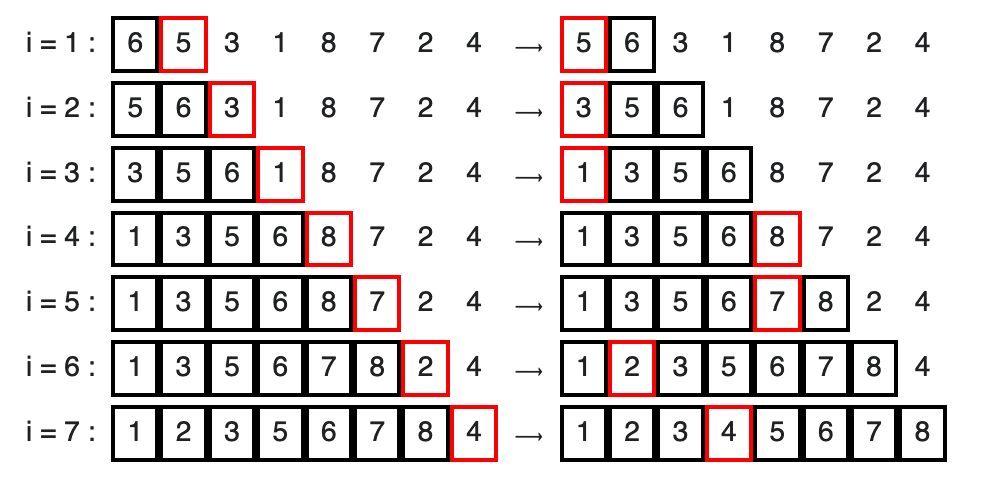
\includegraphics[width=10cm]{ressources/tri_insertion.png}
    \end{figure}
    \ \\
    
    \textbf{Solutions :}
    \begin{itemize}
        \item \textbf{Python :}
                \begin{minted}[fontsize=\footnotesize, autogobble, breaklines]{python}
                    def tri_insertion(l):
                        for i in range(1, len(l)):
                            key = l[i] 
                            j = i-1
                            
                            while j >= 0 and key < l[j] : 
                                    l[j + 1] = l[j] 
                                    j -= 1
                            l[j + 1] = key 
                    
                    if __name__ == "__main__":
                        l = [2, 43, 1, 3, 43]
                        tri_insertion(l)
                        print(l)
                \end{minted}
        \item \textbf{Java :}
                \begin{minted}[fontsize=\footnotesize, autogobble, breaklines]{java}
                    public class Main {
                        public static void tri_insertion(int[] l) {
                            for (int i = 1; i < l.length; i++){
                                int key = l[i]; 
                                int j = i - 1; 
                      
                                while (j >= 0 && l[j] > key) { 
                                    l[j + 1] = l[j]; 
                                    j = j - 1; 
                                } 
                                l[j + 1] = key; 
                            }
                        }
                        
                        public static void printArray(int l[]){ 
                            int n = l.length; 
                            for (int i = 0; i < n; ++i) 
                                System.out.print(l[i] + " "); 
                      
                            System.out.println(); 
                        } 
              
                        
                        public static void main(String[] args){
                            int[] l = {2, 43, 1, 3, 43};
                            tri_insertion(l);
                            printArray(l);
                        }
                    }
                \end{minted}
    \end{itemize}
    
    La complexité de l'algorithme est de $O(n^2)$ car nous utilisons 2 boucles imbriquées, qui dans le pire des cas, parcourent la liste deux fois.
    
\end{Exercice}

\begin{Exercice} [30 minutes] \textbf{Tri fusion (Merge Sort)} \\
    À partir de deux listes triées, on peut facilement construire une liste triée comportant les éléments issus de ces deux listes (leur \textit{fusion}). Le principe de l'algorithme de tri fusion repose sur cette observation : le plus petit élément de la liste à construire est soit le plus petit élément de la première liste, soit le plus petit élément de la deuxième liste. Ainsi, on peut construire la liste élément par élément en retirant tantôt le premier élément de la première liste, tantôt le premier élément de la deuxième liste (en fait, le plus petit des deux, à supposer qu'aucune des deux listes ne soit vide, sinon la réponse est immédiate). 
    
    Les pas de l'algorithme sont comme suit:
    \begin{enumerate}
        \item Si le tableau n'a qu'un élément, il est déjà trié.
        \item Sinon, séparer le tableau en deux parties à peu près égales.
        \item Trier récursivement les deux parties avec l'algorithme du tri fusion.
        \item Fusionner les deux tableaux triés en un seul tableau trié.
    \end{enumerate}
    
    Soit la liste \lstinline{l} suivante, trier les éléments de la liste suivante en utilisant un tri à bulles. Combien d'itération effectuez-vous?
    
    \begin{itemize}
        \item \textbf{Python :}
                \begin{minted}[fontsize=\footnotesize, autogobble, breaklines]{python}
                    def merge(partie_gauche, partie_droite):
                        #TODO: Code à compléter
                    def tri_fusion(l):
                        #TODO: Code à compléter
                    
                    if __name__ == "__main__":
                        l = [38, 27, 43, 3, 9, 82, 10]
                        print(tri_fusion(l))
                \end{minted}
        \item \textbf{Java :}
                \begin{minted}[fontsize=\footnotesize, autogobble, breaklines]{java}
                    public class Main {
                        // Fusionne 2 sous-listes de arr[]. 
                        // Première sous-liste est arr[l..m] 
                        // Deuxième sous-liste est arr[m+1..r] 
                        public static void merge(int arr[], int l, int m, int r) {
                            //TODO: Code à compléter 
                        }
                        
                        // Fonction principale qui trie arr[l..r] en utilisant 
                        // merge() 
                        public static void tri_fusion(int arr[], int l, int r){
                            //TODO: Code à compléter 
                        }
                        
                        public static void printArray(int l[]){ 
                            int n = l.length; 
                            for (int i = 0; i < n; ++i) 
                                System.out.print(arr[i] + " "); 
                      
                            System.out.println(); 
                        } 
              
                        
                        public static void main(String[] args){
                            int[] l = {38, 27, 43, 3, 9, 82, 10};
                            tri_fusion(l);
                            printArray(l);
                        }
                    }
                \end{minted}
    \end{itemize}
    
    \begin{conseil}
    \begin{itemize}
        \item L'algorithme est récursif. 
        \item Revenez à la visualisation de l'algorithme dans les diapositives pour comprendre comment marche concrètement le tri fusion. 
    \end{itemize}
    
    \end{conseil}
    
    \textbf{Solutions :} \\
        \textbf{Python :}
            
            \begin{minted}[fontsize=\footnotesize, autogobble, breaklines]{python}
                def merge(partie_gauche, partie_droite):
                    # créer la liste qui sera retournée à la fin
                    liste_fusionnee = []   
                    
                    # définir un compteur pour l'index de la liste de gauche
                    compteur_gauche = 0   
                    # pareil pour la liste de droite
                    compteur_droite = 0   
                    
                    longueur_gauche = len(partie_gauche)  
                    longueur_droite = len(partie_droite) 
                    
                    # continuer jusqu'à ce que l'un des index (ou les deux) atteigne l'une des longueurs (ou les deux)
                    while compteur_gauche < longueur_gauche and compteur_droite < longueur_droite:
                        # comparer les éléments actuels, ajouter le plus petit à la liste fusionnée 
                        # et augmenter le compteur de cette liste
                        if partie_gauche[compteur_gauche] < partie_droite[compteur_droite]:
                            liste_fusionnee.append(partie_gauche[compteur_gauche])
                            compteur_gauche += 1
                        else:
                            liste_fusionnee.append(partie_droite[compteur_droite])
                            compteur_droite += 1
                    
                    # s'il y a encore des éléments dans les listes, il faut les ajouter à la liste fusionnée
                    liste_fusionnee += partie_gauche[compteur_gauche:longueur_gauche]
                    liste_fusionnee += partie_droite[compteur_droite:longueur_droite]
                    
                    return liste_fusionnee   # retourner la liste fusionnée
                
                def tri_fusion(l):
                    # complèter la fonction
                    longueur = len(l)   # calculer la longueur de la liste
                    # s'il n'y a pas plus d'un élément, retourner la liste
                    if longueur == 1 or longueur == 0:
                        return l
                    # sinon, diviser la liste en deux
                    elif longueur > 1:
                        # convertir la variable en nombre entier (l'index ne peut pas être un nombre à virgule)
                        index_milieu = int(longueur / 2)   
                        # la partie gauche va du 1er élément à celui du milieu
                        partie_gauche = l[0:index_milieu] 
                        # la partie droite va du milieu à la fin de la liste
                        partie_droite = l[index_milieu:longueur]   
                        
                        # appeler la fonction tri_fusion à nouveau sur la partie gauche (récursivité)
                        partie_gauche_triee = tri_fusion(partie_gauche)
                         # même chose pour la partie droite
                        partie_droite_triee = tri_fusion(partie_droite)  
                        
                        liste_fusionnee = merge(partie_gauche_triee, partie_droite_triee)   # enfin, joindre les 2 parties
                        
                        # retourner le résultat
                        return liste_fusionnee   
                
                if __name__ == "__main__":
                        l = [38, 27, 43, 3, 9, 82, 10]
                        print(tri_fusion(l))
    
            \end{minted}
            \textbf{Java :}
            \begin{minted}[fontsize=\footnotesize, autogobble, breaklines]{java}
                public class Main {
                    // Fusionne 2 sous-listes de arr[]. 
                    // Première sous-liste est arr[l..m] 
                    // Deuxième sous-liste est arr[m+1..r] 
                    public static void merge(int arr[], int l, int m, int r) {
                        // Trouver la taille des deux sous-listes à fusionner
                        int n1 = m - l + 1; 
                        int n2 = r - m; 
                  
                        /* Créer des listes temporaires */
                        int L[] = new int[n1]; 
                        int R[] = new int[n2]; 
                  
                        /*Copier les données dans les sous-listes temporaires */
                        for (int i = 0; i < n1; ++i) 
                            L[i] = arr[l + i]; 
                        for (int j = 0; j < n2; ++j) 
                            R[j] = arr[m + 1 + j]; 
                  
                        /* Fusionner les sous-listes temporaires */
                  
                        // Indexes initiaux de la première et seconde sous-liste
                        int i = 0, j = 0; 
                  
                        // Index initial de la sous-liste fusionnée
                        int k = l; 
                        while (i < n1 && j < n2) { 
                            if (L[i] <= R[j]) { 
                                arr[k] = L[i]; 
                                i++; 
                            } 
                            else { 
                                arr[k] = R[j]; 
                                j++; 
                            } 
                            k++; 
                        } 
                  
                        /* Copier les élements restants de L[] */
                        while (i < n1) { 
                            arr[k] = L[i]; 
                            i++; 
                            k++; 
                        } 
                  
                        /* Copier les élements restants de R[] */
                        while (j < n2) { 
                            arr[k] = R[j]; 
                            j++; 
                            k++; 
                        }  
                    }
                    
                    // Fonction principale qui trie arr[l..r] en utilisant 
                    // merge() 
                    public static void tri_fusion(int arr[], int l, int r){
                        if (l < r) { 
                            // Trouver le milieu de la liste
                            int m = (l + r) / 2; 
                  
                            // Trier la première et la deuxième parties de la liste
                            tri_fusion(arr, l, m); 
                            tri_fusion(arr, m + 1, r); 
                  
                            // Fusionner les deux parties
                            merge(arr, l, m, r); 
                        } 
                    }
                    
                    public static void printArray(int l[]){ 
                        int n = l.length; 
                        for (int i = 0; i < n; ++i) 
                            System.out.print(arr[i] + " "); 
                  
                        System.out.println(); 
                    } 
          
                    
                    public static void main(String[] args){
                        int[] l = {38, 27, 43, 3, 9, 82, 10};
                        tri_fusion(l);
                        printArray(l);
                    }
                }
        \end{minted}
        
        Le tri fusion est un algorithme récursif. Ainsi, nous pouvons exprimer la complexité temporelle via une relation de récurence : $T(n) = 2T(n/2) + O(n)$. En effet, l'algorithme comporte 3 étapes :
        \begin{enumerate}
            \item la "Divide Step", qui divise les listes en deux sous-listes, et cela prend un temps constant
            \item la "Conquer Step", qui trie récursivement les sous-listes de taille $n/2$ chacune, et cette étape est représentée par le terme $2T(n/2)$ dans l'équation.
            \item l'étape où l'on fusionne les listes, qui prend $O(n)$.
        \end{enumerate}
        La solution à cette équation est $O(n \log n)$.
\end{Exercice}


\end{document}